% 需要在导言区加载：\usepackage{graphicx,booktabs,float}

\begin{figure}[H]
  \centering
  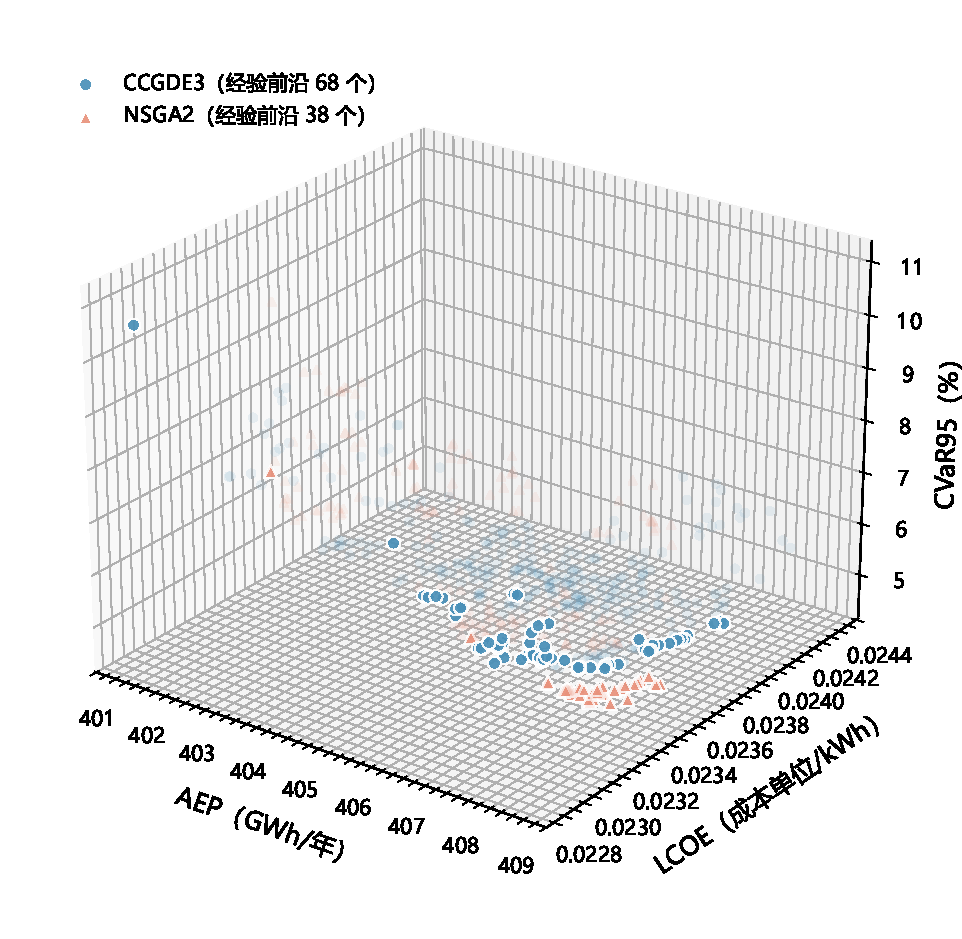
\includegraphics[width=0.88\textwidth]{图表/fig_continuous_pareto_front.pdf}
  \caption{连续坐标版两种算法的三目标最终解集与合并经验 Pareto 前沿。}
  \label{fig:continuous-pareto}
\end{figure}

\begin{figure}[H]
  \centering
  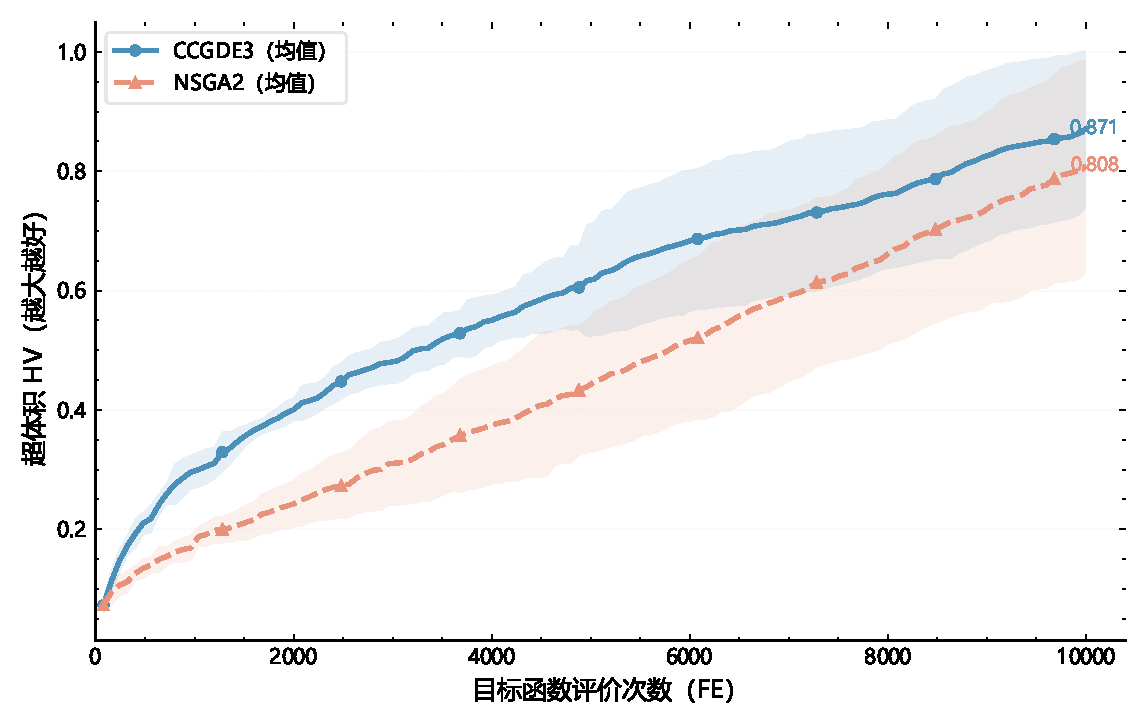
\includegraphics[width=0.84\textwidth]{图表/fig_continuous_convergence_hv.pdf}
  \caption{连续坐标版 HV 收敛过程。曲线为 5 次运行均值，阴影为均值$\pm$1倍标准差。}
  \label{fig:continuous-convergence}
\end{figure}

\begin{figure}[H]
  \centering
  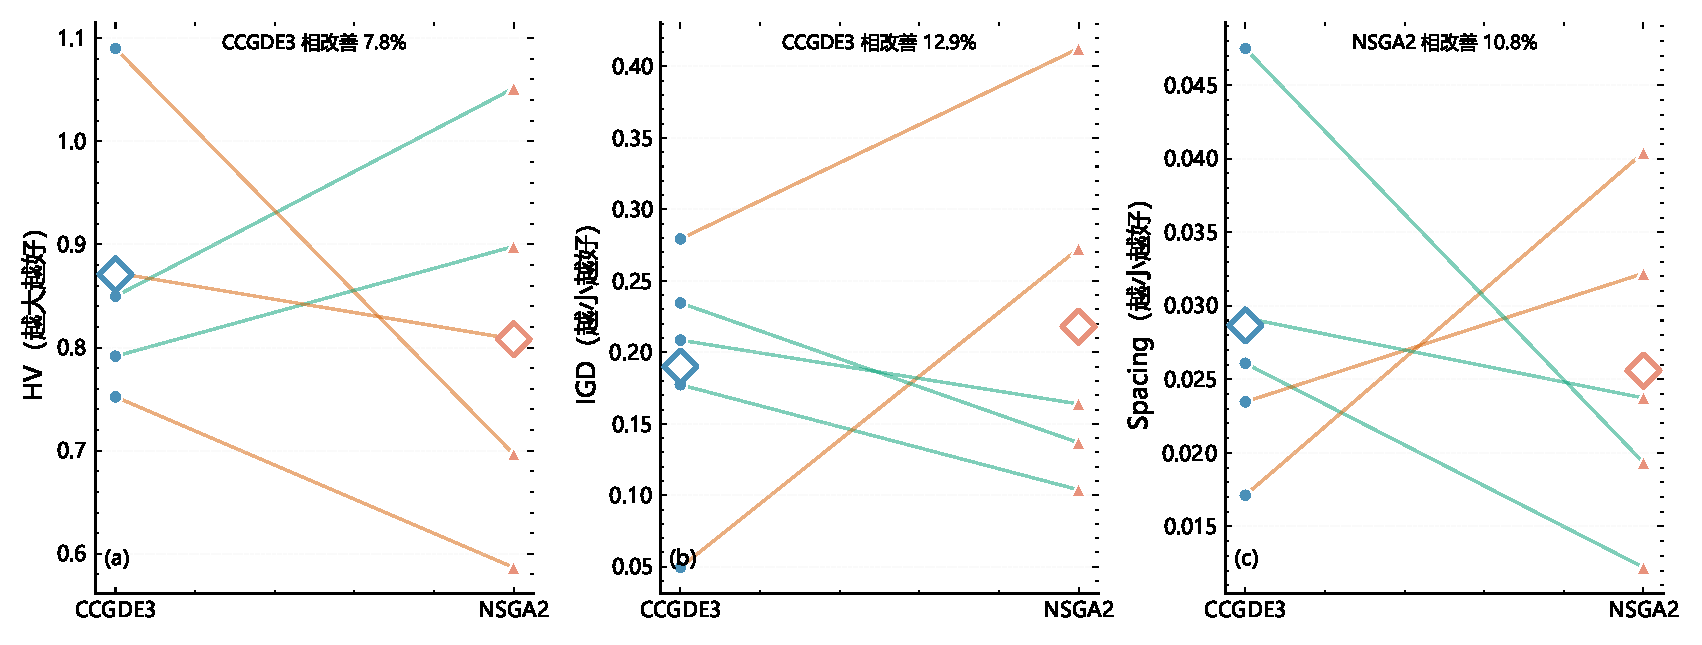
\includegraphics[width=\textwidth]{图表/fig_continuous_metric_distribution.pdf}
  \caption{连续坐标版 5 个随机种子下 HV、IGD 和 Spacing 的配对对比。}
  \label{fig:continuous-metrics}
\end{figure}

\begin{figure}[H]
  \centering
  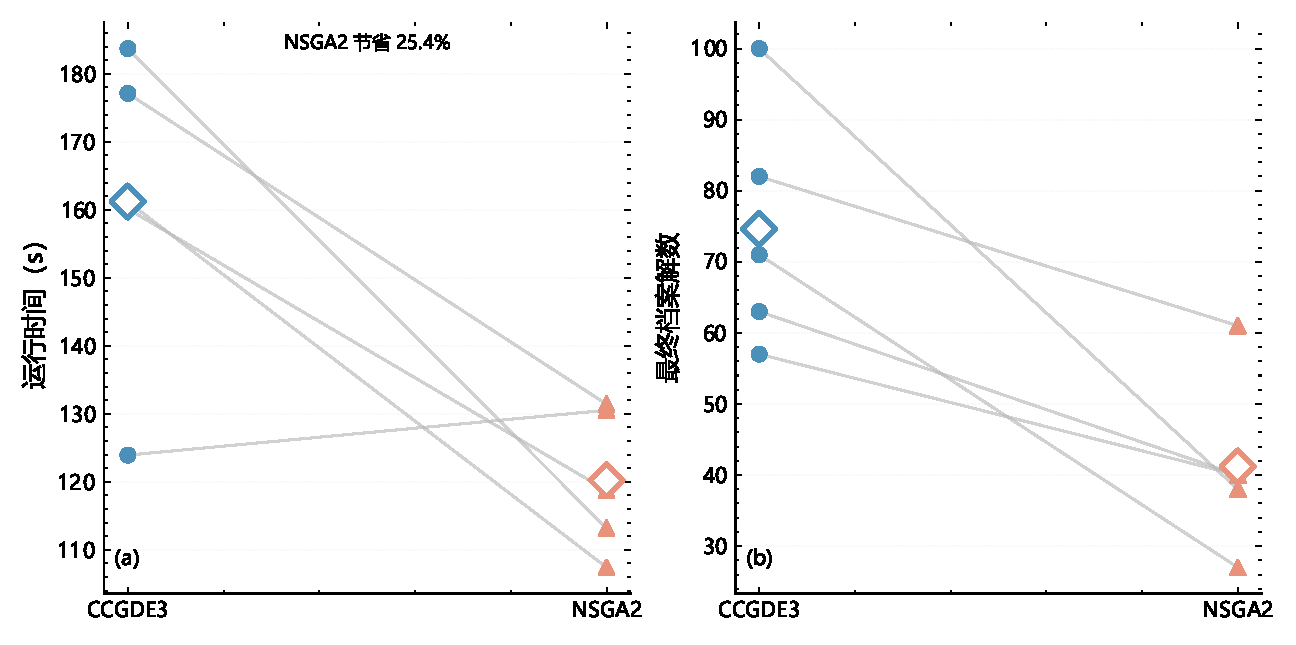
\includegraphics[width=0.90\textwidth]{图表/fig_continuous_runtime.pdf}
  \caption{连续坐标版的运行时间和最终档案规模。}
  \label{fig:continuous-runtime}
\end{figure}

\begin{figure}[H]
  \centering
  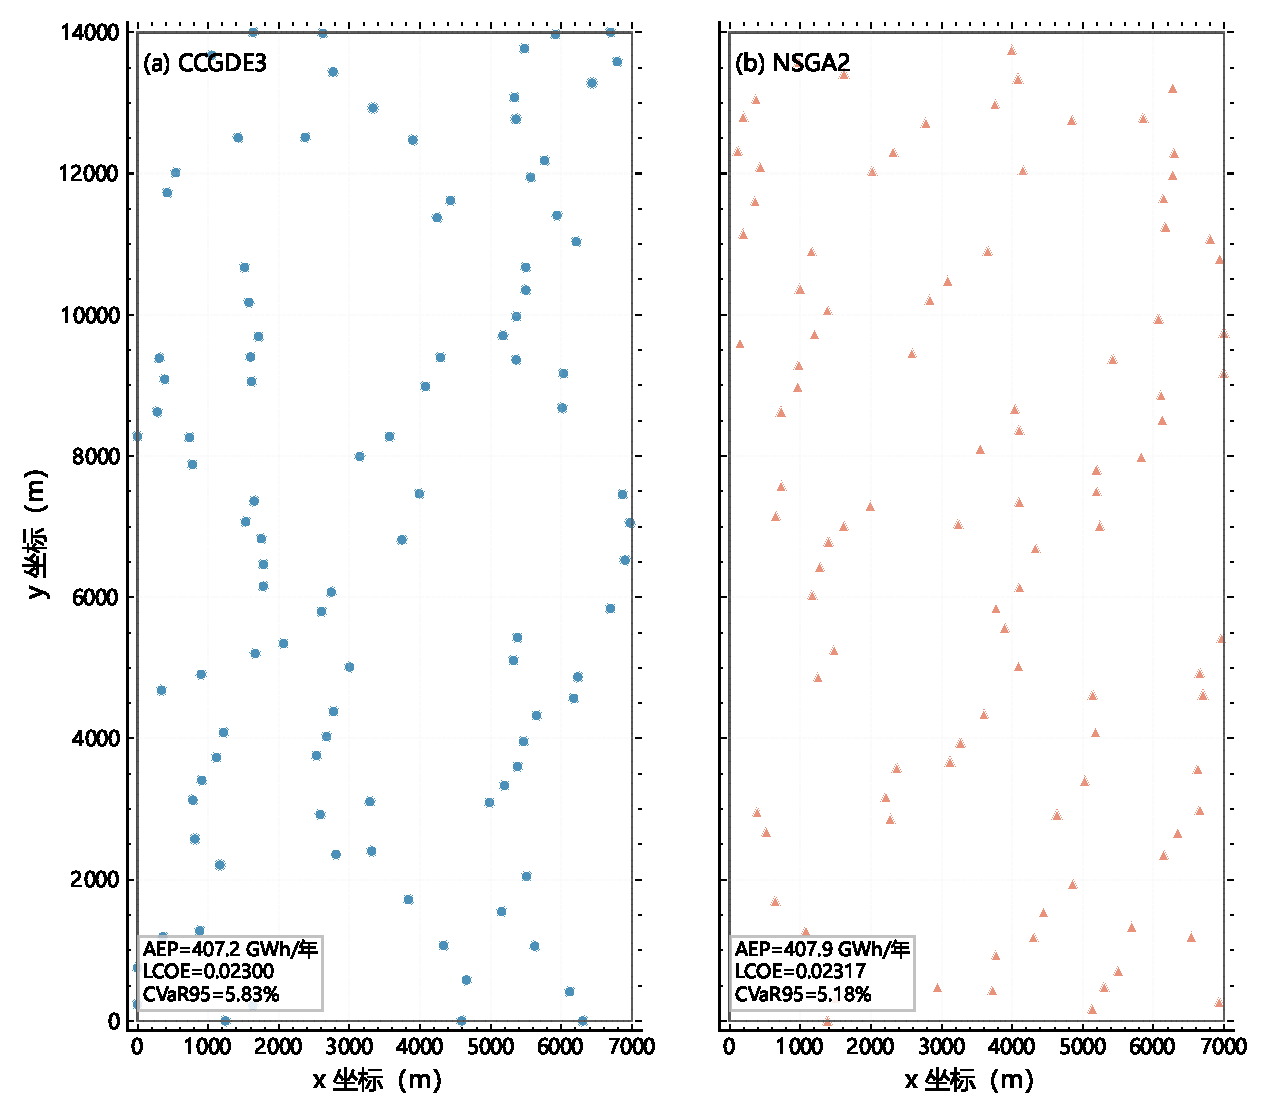
\includegraphics[width=0.90\textwidth]{图表/fig_continuous_layouts.pdf}
  \caption{连续坐标版两种算法代表性折中解的 100 台风机布局。}
  \label{fig:continuous-layouts}
\end{figure}

\begin{figure}[H]
  \centering
  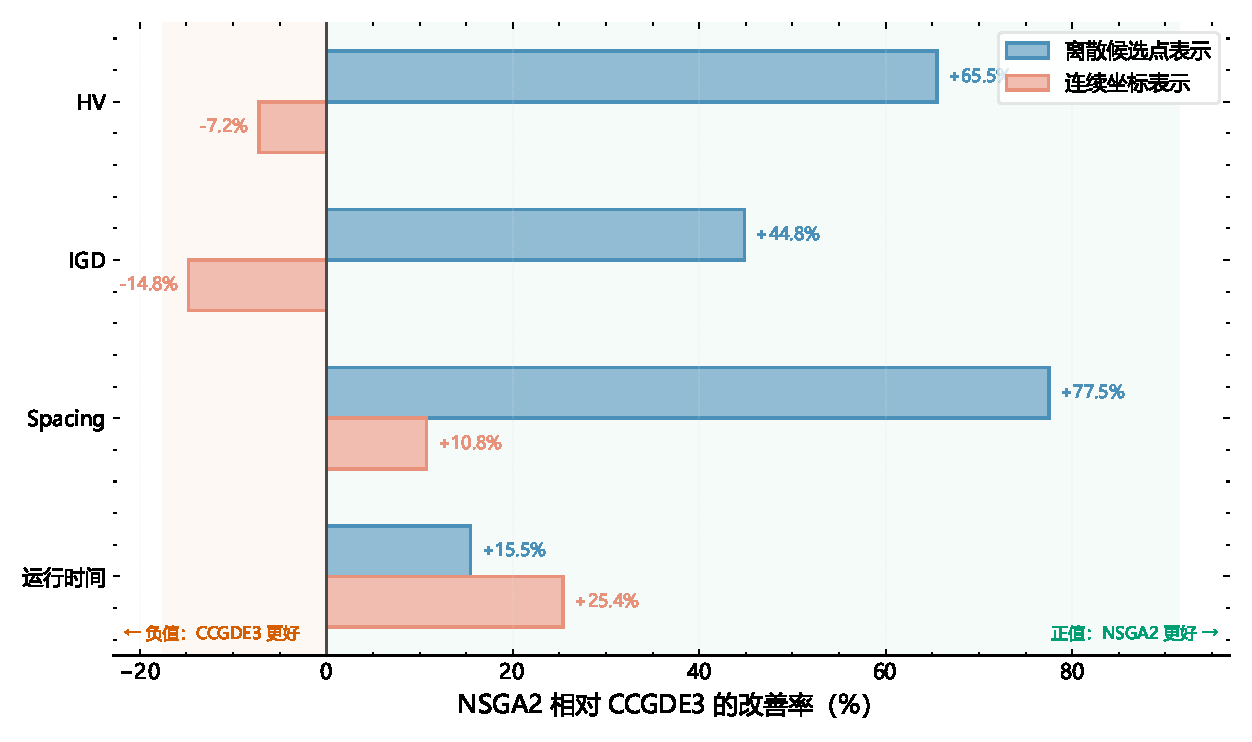
\includegraphics[width=0.92\textwidth]{图表/fig_representation_effect.pdf}
  \caption{离散候选点表示和连续坐标表示下，NSGA2 相对 CCGDE3 的指标改善率。}
  \label{fig:representation-effect}
\end{figure}

\begin{figure}[H]
  \centering
  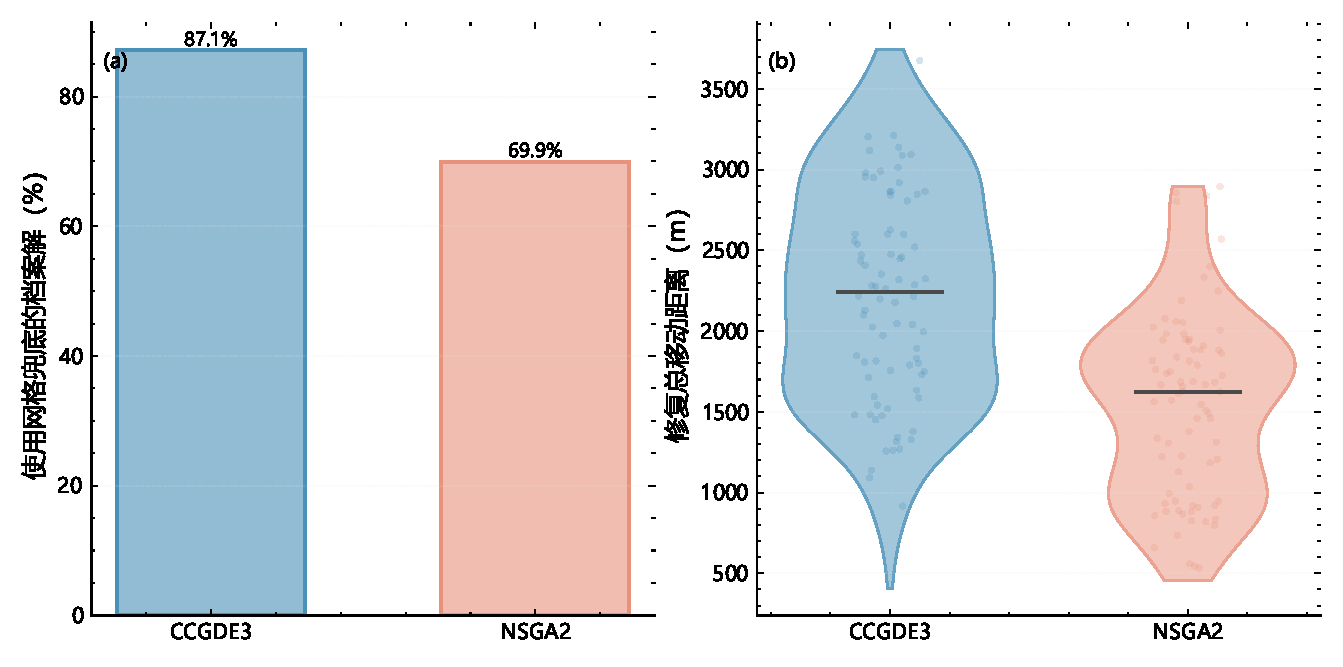
\includegraphics[width=0.92\textwidth]{图表/fig_continuous_repair_diagnostics.pdf}
  \caption{连续布局修复器诊断：网格兜底使用率与修复总移动距离分布。}
  \label{fig:continuous-repair}
\end{figure}

\clearpage
\begin{table}[H]
\centering
\caption{连续变量版算法性能对比（5次独立运行）}
\label{tab:continuous-comparison}
\begin{tabular}{lcccc}
\toprule
算法 & HV$\uparrow$ & IGD$\downarrow$ & Spacing$\downarrow$ & 时间/s$\downarrow$ \\
\midrule
CCGDE3 & 0.8712 $\pm$ 0.1312 & 0.1899 $\pm$ 0.0869 & 0.0287 $\pm$ 0.0114 & 161.22 $\pm$ 23.19 \\
NSGA2 & 0.8082 $\pm$ 0.1793 & 0.2179 $\pm$ 0.1259 & 0.0256 $\pm$ 0.0110 & 120.25 $\pm$ 10.57 \\
\bottomrule
\end{tabular}
\end{table}

\begin{table}[H]
\centering
\caption{连续变量版代表性折中解}
\label{tab:continuous-representatives}
\begin{tabular}{lcccc}
\toprule
算法 & 运行序号 & AEP/(GWh/\text{year}) & LCOE & CVaR95/(\%) \\
\midrule
CCGDE3 & 2 & 407.22 & 0.023000 & 5.83 \\
NSGA2 & 1 & 407.93 & 0.023167 & 5.18 \\
\bottomrule
\end{tabular}
\end{table}


